%% Based on a TeXnicCenter-Template by Gyorgy SZEIDL.
%%%%%%%%%%%%%%%%%%%%%%%%%%%%%%%%%%%%%%%%%%%%%%%%%%%%%%%%%%%%%

%------------------------------------------------------------
%
\documentclass{article}%
%Options -- Point size:  10pt (default), 11pt, 12pt
%        -- Paper size:  letterpaper (default), a4paper, a5paper, b5paper
%                        legalpaper, executivepaper
%        -- Orientation  (portrait is the default)
%                        landscape
%        -- Print size:  oneside (default), twoside
%        -- Quality      final(default), draft
%        -- Title page   notitlepage, titlepage(default)
%        -- Columns      onecolumn(default), twocolumn
%        -- Equation numbering (equation numbers on the right is the default)
%                        leqno
%        -- Displayed equations (centered is the default)
%                        fleqn (equations start at the same distance from the right side)
%        -- Open bibliography style (closed is the default)
%                        openbib
% For instance the command
%           \documentclass[a4paper,12pt,leqno]{article}
% ensures that the paper size is a4, the fonts are typeset at the size 12p
% and the equation numbers are on the left side
%
\usepackage{amsmath}%
\usepackage{amsfonts}%
\usepackage{amssymb}%
\usepackage{graphicx}%
\usepackage{epstopdf}

\addtolength{\textheight}{3.2cm}
\addtolength{\textwidth}{2.6cm}
\addtolength{\marginparwidth}{-2.2cm}
\addtolength{\oddsidemargin}{-1.2cm}
\addtolength{\headheight}{-2.4cm}

%-------------------------------------------
\newtheorem{theorem}{Theorem}
\newtheorem{acknowledgement}[theorem]{Acknowledgement}
\newtheorem{algorithm}[theorem]{Algorithm}
\newtheorem{axiom}[theorem]{Axiom}
\newtheorem{case}[theorem]{Case}
\newtheorem{claim}[theorem]{Claim}
\newtheorem{conclusion}[theorem]{Conclusion}
\newtheorem{condition}[theorem]{Condition}
\newtheorem{conjecture}[theorem]{Conjecture}
\newtheorem{corollary}[theorem]{Corollary}
\newtheorem{criterion}[theorem]{Criterion}
\newtheorem{definition}[theorem]{Definition}
\newtheorem{example}[theorem]{Example}
\newtheorem{exercise}[theorem]{Exercise}
\newtheorem{lemma}[theorem]{Lemma}
\newtheorem{notation}[theorem]{Notation}
\newtheorem{problem}[theorem]{Problem}
\newtheorem{proposition}[theorem]{Proposition}
\newtheorem{remark}[theorem]{Remark}
\newtheorem{solution}[theorem]{Solution}
\newtheorem{summary}[theorem]{Summary}
\newenvironment{proof}[1][Proof]{\textbf{#1.} }{\ \rule{0.5em}{0.5em}}

\begin{document}

\title{Department of  Statistics \\ STATS 784: Data Mining}
\author{Zhi Zhang, $\ $708439475, $\ $zzha822
\\The University of Auckland}
\date{August 16th, 2017}
\maketitle

%\begin{abstract}
%This is a sample document which shows the most important features of the Standard
%\LaTeX\ Journal Article class.
%\end{abstract}

\section{Question 1}
I use the data from "Boston" of library of MASS in R as the input data for the neural network I make myself. \\
\indent And the $\beta_{h}, \sigma$ function and $\alpha_{ih} (i \in {0, 1, 2, \cdots, n})$ are the random numeric generated by R function.\\
\indent "Boston" has 506 records of data, in fact, not all data can give available output based on these random coeffiecients, but some of them can. Below is the first 6 records that can give the output through my own neural network function. For the coeffiecients are random, so every time running the function, the results will be different.
\begin{verbatim}
> mysigmoid = function(x) {
+   exp(x) / (1 + exp(x))
+ }
> 
> neural.net = function(x, alpha, beta, alpha0) {
+   inputs_sum = alpha %*% c(1, x)
+   #print(inputs_sum)
+   blackbox = beta * mysigmoid(inputs_sum)
+   #print(blackbox)
+   sum(blackbox) + alpha0
+ }
> 
> mynnet = function(x, npredict) {
+   alpha = matrix(rep(runif(length(x) + 1), npredict), nrow = npredict)
+   alpha0 = runif(1)
+   beta = runif(npredict)
+   
+   neural.net(x, alpha, beta, alpha0)
+ }
> 
> x = runif(100)
> mynnet(x, 6)
[1] 2.81257
> 
> library(MASS)
> data(Boston)
> 
> samples = data.matrix(Boston[,-ncol(Boston)])
> head(samples)
     crim zn indus chas   nox    rm  age    dis rad tax ptratio  black lstat
1 0.00632 18  2.31    0 0.538 6.575 65.2 4.0900   1 296    15.3 396.90  4.98
2 0.02731  0  7.07    0 0.469 6.421 78.9 4.9671   2 242    17.8 396.90  9.14
3 0.02729  0  7.07    0 0.469 7.185 61.1 4.9671   2 242    17.8 392.83  4.03
4 0.03237  0  2.18    0 0.458 6.998 45.8 6.0622   3 222    18.7 394.63  2.94
5 0.06905  0  2.18    0 0.458 7.147 54.2 6.0622   3 222    18.7 396.90  5.33
6 0.02985  0  2.18    0 0.458 6.430 58.7 6.0622   3 222    18.7 394.12  5.21
> head(apply(samples, 1, function(x) mynnet(x, 6)))
       1        2        3        4        5        6 
2.183425 2.478292 3.787297 2.842076 4.855757 3.418652
\end{verbatim}
Please check R code in a2\_nnet.R. 

%\noindent The front matter has various entries such as\\
%\hspace*{\fill}\verb" \title", \verb"\author", \verb"\date", and
%\verb"\thanks"\hspace*{\fill}\\
%You should replace their arguments with your own.
%
%This text is the body of your article. You may delete everything between the commands\\
%\hspace*{\fill} \verb"\begin{document}" \ldots \verb"\end{document}"
%\hspace*{\fill}\\in this file to start with a blank document.


\section{Question 2}
First we load the Housing Price data from the URL and change variables \emph{\textbf{view}}, and \emph{\textbf{waterf}} to be used as factors for R functions.
\begin{verbatim}
> URL = "https://www.stat.auckland.ac.nz/~lee/784/Assignments/kc_house_data.csv"
> input.df = read.csv(URL)
> names(input.df) = c("id", "date", "price", "bedrooms", "bathrooms",
+ "sqftlv", "sqftlot", "floors", "waterfr", "view",
+ "cond", "grade", "sqfta", "sqftb", "yrb", "yrr",
+ "zip", "lat", "long", "sqftlv15", "sqftlot15")
> head(input.df)
          id            date   price bedrooms bathrooms sqftlv sqftlot floors
1 7129300520 20141013T000000  221900        3      1.00   1180    5650      1
2 6414100192 20141209T000000  538000        3      2.25   2570    7242      2
3 5631500400 20150225T000000  180000        2      1.00    770   10000      1
4 2487200875 20141209T000000  604000        4      3.00   1960    5000      1
5 1954400510 20150218T000000  510000        3      2.00   1680    8080      1
6 7237550310 20140512T000000 1225000        4      4.50   5420  101930      1
  waterfr view cond grade sqfta sqftb  yrb  yrr   zip     lat     long
1       0    0    3     7  1180     0 1955    0 98178 47.5112 -122.257
2       0    0    3     7  2170   400 1951 1991 98125 47.7210 -122.319
3       0    0    3     6   770     0 1933    0 98028 47.7379 -122.233
4       0    0    5     7  1050   910 1965    0 98136 47.5208 -122.393
5       0    0    3     8  1680     0 1987    0 98074 47.6168 -122.045
6       0    0    3    11  3890  1530 2001    0 98053 47.6561 -122.005
  sqftlv15 sqftlot15
1     1340      5650
2     1690      7639
3     2720      8062
4     1360      5000
5     1800      7503
6     4760    101930
>
> input.df$waterfr = factor(input.df$waterfr)
> input.df$view = factor(input.df$view)
> str(input.df)
'data.frame':   21613 obs. of  21 variables:
 $ id       : num  7.13e+09 6.41e+09 5.63e+09 2.49e+09 1.95e+09 ...
 $ date     : Factor w/ 372 levels "20140502T000000",..: 165 221 291 221 
              284 11 57 252 340 306 ...
 $ price    : num  221900 538000 180000 604000 510000 ...
 $ bedrooms : int  3 3 2 4 3 4 3 3 3 3 ...
 $ bathrooms: num  1 2.25 1 3 2 4.5 2.25 1.5 1 2.5 ...
 $ sqftlv   : int  1180 2570 770 1960 1680 5420 1715 1060 1780 1890 ...
 $ sqftlot  : int  5650 7242 10000 5000 8080 101930 6819 9711 7470 6560 ...
 $ floors   : num  1 2 1 1 1 1 2 1 1 2 ...
 $ waterfr  : Factor w/ 2 levels "0","1": 1 1 1 1 1 1 1 1 1 1 ...
 $ view     : Factor w/ 5 levels "0","1","2","3",..: 1 1 1 1 1 1 1 1 1 1 ...
 $ cond     : int  3 3 3 5 3 3 3 3 3 3 ...
 $ grade    : int  7 7 6 7 8 11 7 7 7 7 ...
 $ sqfta    : int  1180 2170 770 1050 1680 3890 1715 1060 1050 1890 ...
 $ sqftb    : int  0 400 0 910 0 1530 0 0 730 0 ...
 $ yrb      : int  1955 1951 1933 1965 1987 2001 1995 1963 1960 2003 ...
 $ yrr      : int  0 1991 0 0 0 0 0 0 0 0 ...
 $ zip      : int  98178 98125 98028 98136 98074 98053 98003 98198 98146 98038 ...
 $ lat      : num  47.5 47.7 47.7 47.5 47.6 ...
 $ long     : num  -122 -122 -122 -122 -122 ...
 $ sqftlv15 : int  1340 1690 2720 1360 1800 4760 2238 1650 1780 2390 ...
 $ sqftlot15: int  5650 7639 8062 5000 7503 101930 6819 9711 8113 7570 ...
\end{verbatim}
Next we transform the target to make it more symmetric, using the Box-Cox transformation.
\begin{verbatim}
> library(caret)
> trans = BoxCoxTrans(input.df$price)
> trans
Box-Cox Transformation

21613 data points used to estimate Lambda

Input data summary:
   Min. 1st Qu.  Median    Mean 3rd Qu.    Max.
  75000  321950  450000  540088  645000 7700000

Largest/Smallest: 103
Sample Skewness: 4.02

Estimated Lambda: -0.2
With fudge factor, Lambda = 0 will be used for transformations

>
> transPrice = predict(trans, input.df$price)
> par(mfrow = c(1, 2))
> hist(input.df$price, main = "Untransformed", nclass = 30)
> hist(transPrice, main = "Transformed", nclass = 30)
\end{verbatim}
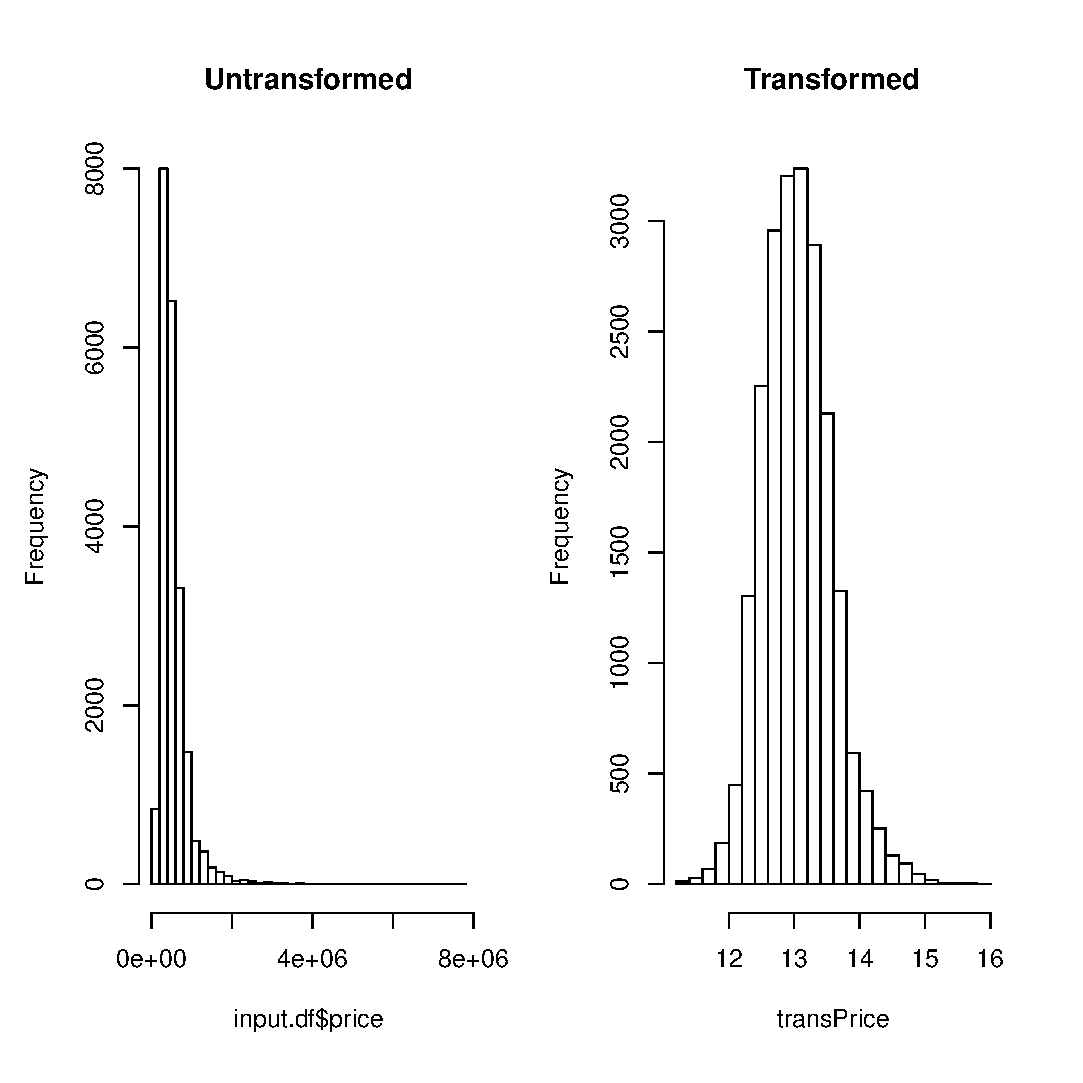
\includegraphics[width=\textwidth]{Symmetric.eps}
From the plot we see that the transformed data is more symmetric, which will get more adavantage to the prediction. We will use transformed  \emph{\textbf{price}} to do the prediction.
\begin{verbatim}
> input.df$price = transPrice
>
> trans = BoxCoxTrans(input.df$sqftlv)
> transSqftlv = predict(trans, input.df$sqftlv)
> input.df$sqftlv = transSqftlv
> trans = BoxCoxTrans(input.df$sqftlot)
> transSqftlot = predict(trans, input.df$sqftlot)
> input.df$sqftlot = transSqftlot
> trans = BoxCoxTrans(input.df$sqftlv15)
> transSqftlv15 = predict(trans, input.df$sqftlv15)
> input.df$sqftlv15 = transSqftlv15
> trans = BoxCoxTrans(input.df$sqftlot15)
> transSqftlot15 = predict(trans, input.df$sqftlot15)
> input.df$sqftlot15 = transSqftlot15
\end{verbatim}
\subsection{Use Neural Network}
Then we will build a non-linear regression model by using neural network to predict the house price. We will use half part of the data as the training set and another half part as the test set. And use the training set to make the prediction model. Pay attention that we remove variables of  \emph{\textbf{id}},  \emph{\textbf{date}},  and \emph{\textbf{zip}} for they make no sense to the regression.\\
\indent First, we use library of caret to tune the parameter of the neural network model, choosing decay from 0.01 and 0.001, and the hidden layer size from 4, 6 and 8. Then we get the best parameter. And pay attention that expand.grid can handle all the variables as factors.
\begin{verbatim}
> used = sample(21613, 10000)
> kingCounty.df = input.df[used,]
> rownames(kingCounty.df) = 1:10000

> library(caret)
> my.grid = expand.grid(.decay = c(0.01, 0.001), .size = c(4, 6, 8))
> nn.CV = train(log(price) ~ bedrooms + bathrooms
+               + sqftlv + sqftlot
+               + floors + waterfr + view + cond + grade 
+               + sqfta + sqftb + yrb + yrr + lat + long
+               + sqftlv15 + sqftlot15, 
+               data = kingCounty.df, 
+               method = "nnet", 
+               maxit = 1000,
+               tuneGrid = my.grid,
+               trace = FALSE,
+               linout = TRUE,
+               trControl = trainControl(method = "cv",
+                                        number = 5,
+                                        repeats = 100))
> 
> nn.CV
Neural Network 

10000 samples
   17 predictor

No pre-processing
Resampling: Cross-Validated (5 fold) 
Summary of sample sizes: 8000, 8000, 8000, 8000, 8000 
Resampling results across tuning parameters:

  decay  size  RMSE        Rsquared 
  0.001  4     0.01990651  0.7539715
  0.001  6     0.01771213  0.8016420
  0.001  8     0.02173159  0.6529491
  0.010  4     0.01836031  0.7869804
  0.010  6     0.01791602  0.7968492
  0.010  8     0.01800531  0.7953671

RMSE was used to select the optimal model using  the smallest value.
The final values used for the model were size = 6 and decay = 0.001.
\end{verbatim}

\indent Next, we use the library of nnet to make the prediction model. Using number of hidden units is 6, and maximum iteration steps are 1000.
\begin{verbatim}
> library(nnet)
> nnet.fit = nnet(log(price) ~ bedrooms + bathrooms
+                 + sqftlv + sqftlot
+                 + floors + waterfr + view + cond + grade 
+                 + sqfta + sqftb + yrb + yrr + lat + long
+                 + sqftlv15 + sqftlot15, 
+                 data = kingCounty.df, size = 6, 
+                 linout = TRUE, decay = 0.001, maxit = 1000)
# weights:  133
initial  value 21347.750583 
iter  10 value 15.619042
iter  20 value 15.394696
iter  30 value 14.689752
iter  40 value 11.113515
iter  50 value 10.924685
iter  60 value 10.915678
iter  70 value 10.908032
iter  80 value 10.332227
iter  90 value 9.239126
iter 100 value 8.860298
iter 110 value 8.114390
iter 120 value 6.361939
iter 130 value 5.742194
iter 140 value 5.170016
iter 150 value 4.461049
iter 160 value 3.963437
iter 170 value 3.882022
iter 180 value 3.809437
iter 190 value 3.738068
iter 200 value 3.708052
iter 210 value 3.657865
iter 220 value 3.613880
iter 230 value 3.561556
iter 240 value 3.524570
iter 250 value 3.497747
iter 260 value 3.493657
iter 270 value 3.469458
iter 280 value 3.444350
iter 290 value 3.437834
iter 300 value 3.436965
iter 310 value 3.414286
iter 320 value 3.373530
iter 330 value 3.370713
iter 340 value 3.345835
iter 350 value 3.257878
iter 360 value 3.224509
iter 370 value 3.214231
iter 380 value 3.212740
iter 390 value 3.210103
iter 400 value 3.201730
iter 410 value 3.192574
iter 420 value 3.184462
iter 430 value 3.174706
iter 440 value 3.168916
iter 450 value 3.166165
iter 460 value 3.165903
iter 470 value 3.160639
iter 480 value 3.149522
iter 490 value 3.129009
iter 500 value 3.128218
iter 510 value 3.126247
iter 520 value 3.120261
iter 530 value 3.110032
iter 540 value 3.088420
iter 550 value 3.069705
iter 560 value 3.055507
iter 570 value 3.045777
iter 580 value 3.039344
iter 590 value 3.034646
iter 600 value 3.032057
iter 610 value 3.031631
iter 620 value 3.031601
iter 630 value 3.029559
iter 640 value 3.026523
iter 650 value 3.022541
iter 660 value 3.014116
iter 670 value 3.004996
iter 680 value 2.999235
iter 690 value 2.995667
iter 700 value 2.991162
iter 710 value 2.977271
iter 720 value 2.967884
iter 730 value 2.965438
iter 740 value 2.964051
iter 750 value 2.962727
iter 760 value 2.961166
iter 770 value 2.960077
iter 780 value 2.957622
iter 790 value 2.954603
iter 800 value 2.951071
iter 810 value 2.947357
iter 820 value 2.942828
iter 830 value 2.938071
iter 840 value 2.934977
iter 850 value 2.932583
iter 860 value 2.928215
iter 870 value 2.924715
iter 880 value 2.923694
iter 890 value 2.923456
iter 900 value 2.920358
iter 910 value 2.915213
iter 920 value 2.906332
iter 930 value 2.897022
iter 940 value 2.876108
iter 950 value 2.857157
iter 960 value 2.846569
iter 970 value 2.839145
iter 980 value 2.833198
iter 990 value 2.829746
iter1000 value 2.827439
final  value 2.827439 
stopped after 1000 iterations
> 
> summary(nnet.fit)
a 20-6-1 network with 133 weights
options were - linear output units  decay=0.001
  b->h1  i1->h1  i2->h1  i3->h1  i4->h1  i5->h1  i6->h1  i7->h1  i8->h1  i9->h1 i10->h1 i11->h1 i12->h1 
  -1.27   -0.01    0.02   -2.76    0.01    0.01   -0.02    0.05    0.03    0.03    0.07    0.03   -0.01 
i13->h1 i14->h1 i15->h1 i16->h1 i17->h1 i18->h1 i19->h1 i20->h1 
   0.00    0.00    0.00    0.01    0.51    0.04   -0.17    0.06 
  b->h2  i1->h2  i2->h2  i3->h2  i4->h2  i5->h2  i6->h2  i7->h2  i8->h2  i9->h2 i10->h2 i11->h2 i12->h2 
  -1.70   -0.01    0.00   -0.35   -0.01    0.16   -0.25    0.10    0.13    0.23    0.07    0.04    0.13 
i13->h2 i14->h2 i15->h2 i16->h2 i17->h2 i18->h2 i19->h2 i20->h2 
   0.00    0.00    0.00    0.02    9.77    3.69   -0.15   -0.04 
  b->h3  i1->h3  i2->h3  i3->h3  i4->h3  i5->h3  i6->h3  i7->h3  i8->h3  i9->h3 i10->h3 i11->h3 i12->h3 
  -0.65    0.00   -0.02   -0.39    0.07    0.00    0.04    0.12    0.10    0.10    0.19    0.02   -0.04 
i13->h3 i14->h3 i15->h3 i16->h3 i17->h3 i18->h3 i19->h3 i20->h3 
   0.00    0.00    0.00    0.41    0.25    0.12   -0.02    0.01 
  b->h4  i1->h4  i2->h4  i3->h4  i4->h4  i5->h4  i6->h4  i7->h4  i8->h4  i9->h4 i10->h4 i11->h4 i12->h4 
  -2.24    0.01    0.01    0.20   -0.05   -0.12    0.24   -0.14   -0.16   -0.22   -0.12   -0.04   -0.03 
i13->h4 i14->h4 i15->h4 i16->h4 i17->h4 i18->h4 i19->h4 i20->h4 
   0.00    0.00    0.00    0.00   -7.28   -2.85    0.21   -0.01 
  b->h5  i1->h5  i2->h5  i3->h5  i4->h5  i5->h5  i6->h5  i7->h5  i8->h5  i9->h5 i10->h5 i11->h5 i12->h5 
   2.05    0.01   -0.02   -0.09    0.00   -0.01   -0.10   -0.02   -0.01   -0.02    0.01    0.00   -0.04 
i13->h5 i14->h5 i15->h5 i16->h5 i17->h5 i18->h5 i19->h5 i20->h5 
   0.00    0.00    0.00    0.00   -0.69   -0.25   -0.04    0.01 
  b->h6  i1->h6  i2->h6  i3->h6  i4->h6  i5->h6  i6->h6  i7->h6  i8->h6  i9->h6 i10->h6 i11->h6 i12->h6 
   0.00    0.01    0.00    0.00    0.03    0.00    0.00    0.00    0.00    0.00    0.00   -0.04    0.00 
i13->h6 i14->h6 i15->h6 i16->h6 i17->h6 i18->h6 i19->h6 i20->h6 
  -0.23   -0.06    0.05    0.02   -0.04    0.07    0.00    0.01 
 b->o h1->o h2->o h3->o h4->o h5->o h6->o 
 0.85  0.64  0.65  0.83  0.87 -1.75  0.03 
> 
> RSS = sum(residuals(nnet.fit)^2)
> RSS.null = sum((log(input.df$price) - mean(log(input.df$price)))^2)
> R2 = 1 - RSS/RSS.null
> 
> RSS
[1] 2.627252
> RSS.null
[1] 34.77776
> R2
[1] 0.924456
> 
\end{verbatim}

We get apparent error and the test set error as below:
\begin{verbatim}
> mean(residuals(nnet.fit)^2)
[1] 0.0002627252
> 
> newKingCounty.df = input.df[-used,]
> rownames(newKingCounty.df) = 1:11613
> predictions = predict(nnet.fit, newdata = newKingCounty.df)
> 
> actuals = log(newKingCounty.df$price)
> mean((predictions - actuals)^2)
[1] 0.0002723154
\end{verbatim}

Furthermore, we use CV and bootstrap methods in caret libary to tune the parameter again to validate if our previous choice is really good.
\begin{verbatim}
> my.grid = expand.grid(.decay = c(0.01, 0.001), .size = c(6, 8, 10))
> CV10.NN = train(log(price)~ bedrooms + bathrooms
+              + sqftlv + sqftlot + floors 
+              + waterfr + view + cond + grade 
+              + sqfta + sqftb + yrb + yrr + lat + long
+              + sqftlv15 + sqftlot15,
+              data = kingCounty.df,
+              method = "nnet", 
+              maxit = 1000,
+              tuneGrid = my.grid,
+              trace = FALSE,
+              linout = TRUE,
+              trControl = trainControl(method = "cv", 
+                                       number = 10, 
+                                       repeats = 100))
> CV10.NN
Neural Network 

10000 samples
   17 predictor

No pre-processing
Resampling: Cross-Validated (10 fold) 
Summary of sample sizes: 9001, 9001, 8999, 9000, 9001, 8999, ... 
Resampling results across tuning parameters:

  decay  size  RMSE        Rsquared 
  0.001   6    0.02031734  0.7101410
  0.001   8    0.01830722  0.7879843
  0.001  10    0.01914487  0.7781375
  0.010   6    0.01785190  0.7986983
  0.010   8    0.01742965  0.8081612
  0.010  10    0.01760189  0.8043962

RMSE was used to select the optimal model using  the smallest value.
The final values used for the model were size = 8 and decay = 0.01. 
> 
> boot.NN = train(log(price)~ bedrooms + bathrooms
+              + sqftlv + sqftlot + floors 
+              + waterfr + view + cond + grade 
+              + sqfta + sqftb + yrb + yrr + lat + long
+              + sqftlv15 + sqftlot15,
+              data = kingCounty.df,
+              method = "nnet", 
+              maxit = 1000,
+              tuneGrid = my.grid,
+              trace = FALSE,
+              linout = TRUE,
+              trControl = trainControl(method = "boot", 
+                                       repeats = 200))
Warning message:
In nominalTrainWorkflow(x = x, y = y, wts = weights, info = trainInfo,  :
  There were missing values in resampled performance measures.
> boot.NN
Neural Network 

10000 samples
   17 predictor

No pre-processing
Resampling: Bootstrapped (25 reps) 
Summary of sample sizes: 10000, 10000, 10000, 10000, 10000, 10000, ... 
Resampling results across tuning parameters:

  decay  size  RMSE        Rsquared 
  0.001   6    0.02240144  0.6861685
  0.001   8    0.01759080  0.8038163
  0.001  10    0.01819424  0.7913595
  0.010   6    0.01798248  0.7954653
  0.010   8    0.01792334  0.7969508
  0.010  10    0.01835575  0.7886608

RMSE was used to select the optimal model using  the smallest value.
The final values used for the model were size = 8 and decay = 0.001. 
\end{verbatim}

\indent Different from the previous choice, this time it indicate choose size of 8 and decay of 0.01 or 0.001, but the RMSE in fact is similar to our previous choice, so they should be most similar to the prediction results.\\
\indent The accuracy is pretty good when using neural network model. The prediction error is about 0.00027, which is obviously lower than the linear regression model.

\subsection{Use Regression Tree}
Now



\end{document}
